\chapter{Testing in Scratch}

\chapter{Background and Related Work}

=== Scratch
- block based programming language
- code controls sprites on a two-dimensional stage
- creates a interactive animated project

\begin{wrapfigure}{r}{0.5\textwidth}
    \centering
    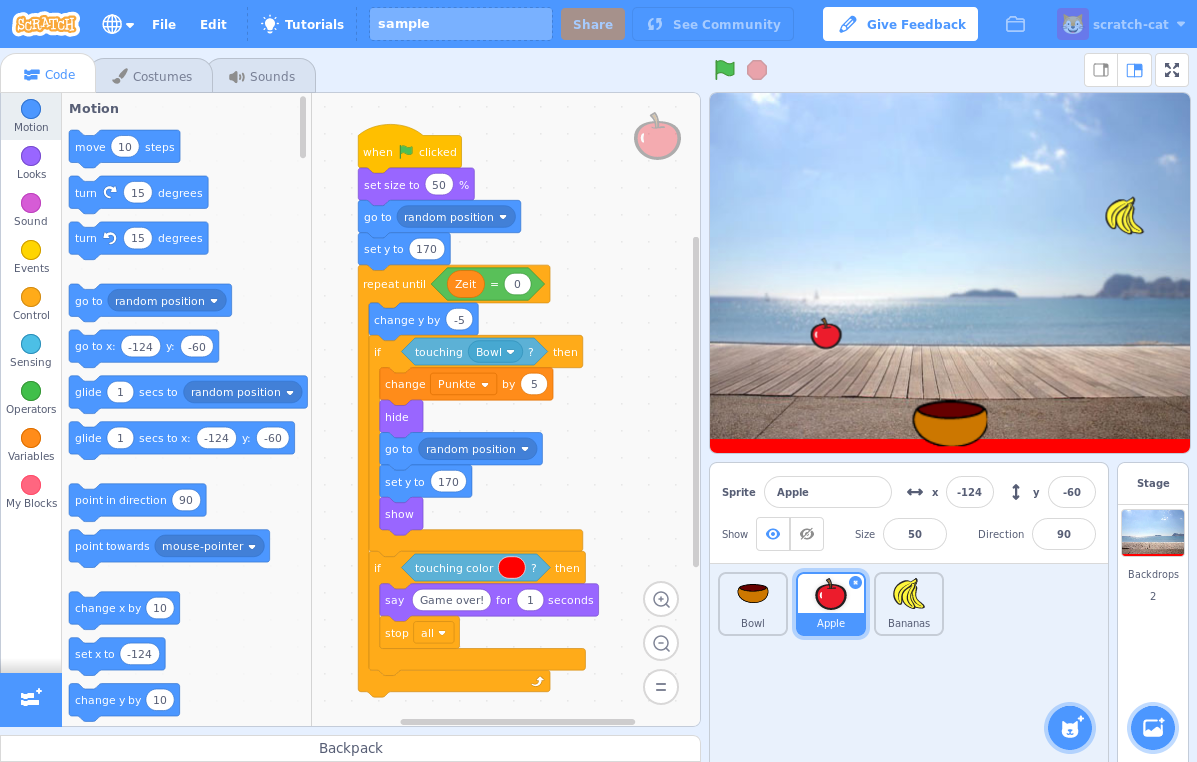
\includegraphics[width=0.4\textwidth]{scratch-example}
    \caption{Scratch Interface}
    \label{fig:scratch_interface}
\end{wrapfigure}

- attractive because ...
    - it eliminates syntax errors
    - is intuitive, e.g. all possible blocks are available from a drawer, no documentation needed
    - facilitates creativity
    - very easy to execute project or parts of the project -> prototyping approach

- However, automatic assessment of Scratch programs is still an open problem
- At least two other projects have tackled the task of automatically assessing Scratch projects.

=== Hairball
- Hairball \cite{hairball} allows static analysis of scratch programs
- Good way to check if certain constructs are used in a project
    - Allows to check if students use a new construct, which the exercise focuses on
- Allows to detect code smells
- Allows to measure the complexity of a program -> see Dr.Scratch
- Not suitable to check the functionality of a program

=== ITCH
- ITCH (Individual Testing of Computer Homework for Scratch Assignments) \cite{itch}
- ITCH allows simple textual input, output testing using "ask" and "say" blocks
- This, however,  only allows to test projects with a small subset of Scratch functionality
- Not very useful in general for Scratch because it focuses on multimedia and creativity

\section{Approach}
- Scratch Programs are hard to analyze
    - use of multimedia
    - lack of a main entry point
    - executed by running multiple parallel scripts

- Whisker follows an approach which is a bit similar to GUI Testing
- Complete black box approach
- Simulate user input and check the result
- One test executes the program exactly once

- Whisker should be used together with manual analysis (and maybe static analysis like Hairball if fully automated grading is the goal)
